\section{Wyniki}

Niniejsza sekcja przedstawia i porównuje wyniki otrzymane w eksperymencie. Metody wchodzące w skład porównania to "Delayed Column Generation" (\hyperref[sec:dcg]{rozdział~\ref*{sec:dcg}}) oraz "Brutal Force" (\hyperref[brutalForce]{rozdział~\ref*{brutalForce}}). Warunki przeprowadzenia testu:
\begin{itemize}
  \item Losowo generowane odcinki wynikowe o długości od 1 do 21 cm, przy liczebności od 1 do 200 elementów.
  \item Losowo generowane 5 długości początkowych od 22 do 42 cm, o koszcie od 1\$. Każda długość posiada inną cenę.
  \item Obie metody testowane są z tymi samymi danymi.
  \item Wykonano 28 różnych rozkrojów.
  \item Czas wykonania mierzony od dostarczenia danych do zwrócenia wyniku, bez uwzględnianienia czasu przygotowania danych oraz ich zapisu.
  \item Warunki sprzętowe:
  \begin{itemize}
    \item Procesor: Intel Core i5-6500u @ 2.30 GHz x 2 z technologią HT.
    \item RAM: 16 GB (15.2 GB).
    \item System operacyjny: Linux Mint 18.1 Cinammon 64-bit.
  \end{itemize}
  \item Język implementacji: Kotiln 1.0.5 (JVM), Java 8 (Oracle Java 1.8\_121).
  \item Aplikacja jednowątkowa.
\end{itemize}
\subsection{Porównanie}

Dane z tabeli \ref{tab:result} przedstawiają porównanie podstawowych statystyk dla każdego kroku eksperymentu. Natomiast tabela \ref{tab:average} przedstawia średnie wartości statystyk przedstawionych w tabeli ją poprzedzającej.

\begin{table}[]
\centering
\caption{Wyniki}
\label{tab:result}
\begin{tabular}{@{}|c|c|c|c|c|c|@{}}
\toprule
\multicolumn{2}{|c|}{\textbf{Czas (ms)}} & \multicolumn{2}{c|}{\textbf{Koszt}} & \multicolumn{2}{c|}{\textbf{Odpad}} \\ \midrule
\textit{DCG}        & \textit{BF}        & \textit{DCG}      & \textit{BF}     & \textit{DCG}      & \textit{BF}     \\ \midrule
136396              & 11                 & 1830              & 2835            & 0                 & 0               \\ \midrule
27688               & 2                  & 1719              & 2342            & 304               & 13              \\ \midrule
190893              & 3                  & 3279              & 3421            & 109               & 33              \\ \midrule
113044              & 2                  & 1936              & 5397            & 69                & 20              \\ \midrule
14453               & 5                  & 1821              & 2342            & 819               & 8               \\ \midrule
446814              & 1                  & 2912              & 4254            & 3947              & 3               \\ \midrule
20758               & 3                  & 4544              & 5050            & 1729              & 3               \\ \midrule
101468              & 2                  & 3024              & 6658            & 54                & 1               \\ \midrule
272598              & 1                  & 2324              & 2560            & 44                & 0               \\ \midrule
18424               & 1                  & 2365              & 4001            & 877               & 64              \\ \midrule
284007              & 1                  & 1802              & 4000            & 46                & 40              \\ \midrule
36820               & 6                  & 3078              & 3255            & 393               & 115             \\ \midrule
25840               & 8                  & 4068              & 6981            & 325               & 14              \\ \midrule
42254               & 16                 & 948               & 1034            & 1480              & 102             \\ \midrule
4664                & 1                  & 3174              & 3707            & 1434              & 1297            \\ \midrule
11725               & 3                  & 1377              & 2904            & 46                & 2               \\ \midrule
34074               & 6                  & 1161              & 1490            & 411               & 45              \\ \midrule
323568              & 7                  & 3072              & 3638            & 81                & 1               \\ \midrule
124059              & 4                  & 8128              & 8971            & 0                 & 51              \\ \midrule
27697               & 1                  & 830               & 3965            & 0                 & 9               \\ \midrule
169184              & 2                  & 2754              & 3255            & 0                 & 18              \\ \midrule
227189              & 7                  & 3184              & 5741            & 150               & 94              \\ \midrule
25436               & 5                  & 1235              & 1850            & 35                & 21              \\ \midrule
232145              & 3                  & 4485              & 4598            & 0                 & 4               \\ \midrule
47524               & 2                  & 2993              & 4046            & 1278              & 159             \\ \midrule
77913               & 2                  & 5002              & 5196            & 23                & 10              \\ \midrule
201725              & 1                  & 2366              & 3162            & 0                 & 14              \\ \midrule
18760               & 2                  & 5330              & 5398            & 64                & 12              \\ \bottomrule
\end{tabular}
\end{table}

\begin{table}[]
\centering
\caption{Średnie}
\label{tab:average}
\begin{tabular}{|l|c|c|}
\hline
                                           & \textbf{DCG}   & \textbf{BF}   \\ \hline
\textbf{Średni czas}                       & 116325.71      & 3.86          \\ \hline
\textbf{(DCG/BF) * 100\%}  & \multicolumn{2}{c|}{3015851.85\%} \\ \hline
\textbf{Średni koszt}                      & 2883.61        & 4001.82       \\ \hline
\textbf{(BF/DCG) * 100\%} & \multicolumn{2}{c|}{138.78\%}  \\ \hline
\textbf{Średni odpad}                      & 489.93         & 76.89         \\ \hline
\textbf{(DCG/BF) * 100\%} & \multicolumn{2}{c|}{637.16\%}    \\ \hline
\end{tabular}
\end{table}

Dane przedstawione w tabelach \ref{tab:result} oraz \ref{tab:average} wskzaują jednoznacznie że, metoda brutalnej siły (dalej BF) jest szybsza niż druga metoda użyta w porównaniu. Tabela \ref{tab:average} wskazuje iż metoda opóźnionej generacji kolumn (dalej DCG) jest prawie 30156 razy wolniejsza niż metoda BF. Ma to związek z nakładem obliczeniowym metody DCG. Metoda ta wykonuje wiele obliczeń macierzowych, dla każdej itereacji zachodzi odwracanie macierzy, mnożenie wektorów, eliminacja Gaussa oraz rozwiązywanie układu nierówności dwufazową metodą sympleks. Najwyższy czas wykonania metody DCG wynosi 446814 ms, czyli ponad 7 minut. Najmniejszy czas wykonania tej samej metody przy innych danych wejściowych i zachowaniu warunków testu wynosi 4664 ms, czyli 4,7 s. Rozbieżność czasów wykonania metody DCG wskazują na silną zależność między danymi wejściowymi, a czasem wykonania. Czas wykonania metody BF jest bardzo niski, na poziomie kilkunastu milisekund, jest to związane ze spsobem implementacji. Głównym elementem tej metody jest przeszukiwanie, przechodzenie oraz uzupełnianie tablic. Operacje te są znacznie szybsze niż operacje macierzowe. Mediana czasów obu metod pokazuje że, metoda DCG nadal jest dużo wolniejsza niż BF, jednak w innej skali niż porównanie średnich. Mediana dla metody DCG to 62718.5 ms, a dla BF to 2.5 s. Metoda DCG jest ponad 25087 razy wolniejsza niż metoda BF.

Kolejna część tabel odnosi się do średniego kosztu wykroju całkowitego. Koszt uzyskany metodą BF jest średnio 1.4 razy większy niż metodą DCG. Stosunek kosztu metody pierwszej oraz drugej jest relatywnie niski. Jednak po sprawdzeniu wielkości kosztów wynika iż, różnica między ceną rozwiązania metodą DCG oraz metodą BF wynosi 1118,21\$. Rząd wielkości oznacza że, różnica w cenie jest znacząca. Metoda DCG jako główny cel przyjmuje minimalizację kosztu, natomiast metoda BF jak najmniejszą cenę odpadu w ujęciu bierzącecgo schematu rozkroju.

Końcowe częsci tabel ukazują odpad powstały z rozkroju otrzymanymi schmatami. Odpad wyprodukowany z metody DCG jest ponad 6 razy większy niż odpad z metdoy BF. W jednym przypadku na 28, odpad z metdy DCG był mniejszy niż z metody BF. Tak jak zostało wspomnianie w powyższym akapicie metoda BF skupia się na minimalizacji kosztu odpadu, w uogólnionym przypadku minimalizuje odpad.   

Zgdodnie z eksperymentem przeprowadzonym przez Gilmorea oraz Gomorego \cite{GilmoreGomoryV2Article}, prawdą jest że, im szybciej metoda zakończy obliczenia, tym większy będzie odpad. Trend ten jest zauważalny w tabeli \ref{tab:result}.

Poniższe tabele \ref{tab:dcg_result} oraz \ref{tab:bf_result} prezentują wynik jednego wywołania metody opóźnionej generacji kolumn oraz metody brutalnej siły.

\clearpage
\begin{longtable}{lllllllll}
\caption{Rezultat DCG}\label{tab:dcg_result} \\
\hline \\
Wejście                   &              &           &                  &    &    &    &   &    \\
Podstawa             &              &           &                  &    &    &    &   &    \\
Długość                   & Koszt         &           &                  &    &    &    &   &    \\
25                       & 7            &           &                  &    &    &    &   &    \\
31                       & 21           &           &                  &    &    &    &   &    \\
33                       & 9            &           &                  &    &    &    &   &    \\
36                       & 15           &           &                  &    &    &    &   &    \\
Zamówienie     &              &           &                  &    &    &    &   &    \\
Długość                   & Koszt     &           &                  &    &    &    &   &    \\
2                        & 66           &           &                  &    &    &    &   &    \\
4                        & 167          &           &                  &    &    &    &   &    \\
5                        & 174          &           &                  &    &    &    &   &    \\
7                        & 151          &           &                  &    &    &    &   &    \\
9                        & 200          &           &                  &    &    &    &   &    \\
10                       & 135          &           &                  &    &    &    &   &    \\
12                       & 150          &           &                  &    &    &    &   &    \\
15                       & 26           &           &                  &    &    &    &   &    \\
17                       & 8            &           &                  &    &    &    &   &    \\
                         &              &           &                  &    &    &    &   &    \\
Wyjście                   &              &           &                  &    &    &    &   &    \\
Użyte podstawy         &              &           &                  &    &    &    &   &    \\
Długość                   & Ilość     &           &                  &    &    &    &   &    \\
25                       & 305          &           &                  &    &    &    &   &    \\
33                       & 21           &           &                  &    &    &    &   &    \\
                         &              &           &                  &    &    &    &   &    \\
Rozkroje             &              &           &                  &    &    &    &   &    \\
Ilość                 & Odpad        & Podstawa & \multicolumn{6}{c}{Schemat}    \\
14                       & 0            & 25        & 2                & 2  & 2  & 2  & 5 & 12 \\
76                       & 0            & 25        & 4                & 4  & 5  & 12 &   &    \\
4                        & 0            & 25        & 5                & 5  & 5  & 5  & 5 &    \\
16                       & 0            & 25        & 4                & 7  & 7  & 7  &   &    \\
96                       & 0            & 25        & 7                & 9  & 9  &    &   &    \\
68                       & 0            & 25        & 5                & 10 & 10 &    &   &    \\
31                       & 1            & 25        & 12               & 12 &    &    &   &    \\
13                       & 1            & 33        & 2                & 15 & 15 &    &   &    \\
8                        & 0            & 33        & 7                & 9  & 17 &    &   &    \\
                         &              &           &                  &    &    &    &   &    \\
Statystyka                &              &           &                  &    &    &    &   &    \\
Czas (ms)           & 272598       &           &                  &    &    &    &   &    \\
Koszt               & 2324         &           &                  &    &    &    &   &    \\
Odpad                    & 44           &           &                  &    &    &    &   &    \\
Odpad \%            & 5.289733E-05 &           &                  &    &    &    &   &    \\
                         &              &           &                  &    &    &    &   &    \\
Wynik         &              &           &                  &    &    &    &   &    \\
Długość                   & Ilość     &           &                  &    &    &    &   &    \\
2                        & 69           &           &                  &    &    &    &   &    \\
4                        & 168          &           &                  &    &    &    &   &    \\
5                        & 178          &           &                  &    &    &    &   &    \\
7                        & 152          &           &                  &    &    &    &   &    \\
9                        & 200          &           &                  &    &    &    &   &    \\
10                       & 136          &           &                  &    &    &    &   &    \\
12                       & 152          &           &                  &    &    &    &   &    \\
15                       & 26           &           &                  &    &    &    &   &    \\
17                       & 8            &           &                  &    &    &    &   &    \\
                         &              &           &                  &    &    &    &   &    \\
Spadek kosztu &              &           &                  &    &    &    &   &    \\
Krok                     & Koszt         &           &                  &    &    &    &   &    \\
0                        & 2755.0166    &           &                  &    &    &    &   &    \\
1                        & 2692.1833    &           &                  &    &    &    &   &    \\
2                        & 2661.5166    &           &                  &    &    &    &   &    \\
3                        & 2437.5166    &           &                  &    &    &    &   &    \\
4                        & 2343.0166    &           &                  &    &    &    &   &    \\
5                        & 2324.7388    &           &                  &    &    &    &   &    \\
6                        & 2317.6765    &           &                  &    &    &    &   &    \\
7                        & 2314.585     &           &                  &    &    &    &   &    \\
8                        & 2303.9917    &           &                  &    &    &    &   & \\
\hline
\end{longtable}

\clearpage
\begin{longtable}{llllllllllll}
  \caption{Rezultat BF}\label{tab:bf_result} \\
  \hline \\
  Wyjście               &          &           &                  &    &    &   &   &   &   &   &   \\
  Użyte podstawy     &          &           &                  &    &    &   &   &   &   &   &   \\
  Długość               & Ilość &           &                  &    &    &   &   &   &   &   &   \\
  25                   & 94       &           &                  &    &    &   &   &   &   &   &   \\
  33                   & 113      &           &                  &    &    &   &   &   &   &   &   \\
  36                   & 59       &           &                  &    &    &   &   &   &   &   &   \\
                       &          &           &                  &    &    &   &   &   &   &   &   \\
  Rozkroje         &          &           &                  &    &    &   &   &   &   &   &   \\
  Ilość             & Odpad    & Podstawa &  \multicolumn{9}{c}{Schemat} \\
  4                    & 0        & 36        & 17               & 17 & 2  &   &   &   &   &   &   \\
  25                   & 0        & 25        & 15               & 10 &    &   &   &   &   &   &   \\
  1                    & 0        & 36        & 15               & 12 & 9  &   &   &   &   &   &   \\
  74                   & 0        & 33        & 12               & 12 & 9  &   &   &   &   &   &   \\
  1                    & 0        & 36        & 12               & 10 & 10 & 4 &   &   &   &   &   \\
  53                   & 0        & 25        & 10               & 10 & 5  &   &   &   &   &   &   \\
  1                    & 0        & 33        & 10               & 10 & 9  & 4 &   &   &   &   &   \\
  31                   & 0        & 36        & 9                & 9  & 9  & 9 &   &   &   &   &   \\
  37                   & 0        & 33        & 7                & 7  & 7  & 7 & 5 &   &   &   &   \\
  1                    & 0        & 33        & 7                & 7  & 7  & 5 & 5 & 2 &   &   &   \\
  16                   & 0        & 25        & 5                & 5  & 5  & 5 & 5 &   &   &   &   \\
  1                    & 0        & 36        & 5                & 5  & 4  & 4 & 4 & 4 & 4 & 4 & 2 \\
  17                   & 0        & 36        & 4                & 4  & 4  & 4 & 4 & 4 & 4 & 4 & 4 \\
  1                    & 0        & 36        & 4                & 4  & 4  & 4 & 4 & 4 & 2 & 2 & 2 \\
                       &          &           & 2                & 2  & 2  &   &   &   &   &   &   \\
  3                    & 0        & 36        & 2                & 2  & 2  & 2 & 2 & 2 & 2 & 2 & 2 \\
                       &          &           & 2                & 2  & 2  & 2 & 2 & 2 & 2 & 2 & 2 \\
                       &          &           &                  &    &    &   &   &   &   &   &   \\
  Statystyka            &          &           &                  &    &    &   &   &   &   &   &   \\
Czas (ms)       & 1        &           &                  &    &    &   &   &   &   &   &   \\
  Koszt           & 2560     &           &                  &    &    &   &   &   &   &   &   \\
  Odpad                & 0        &           &                  &    &    &   &   &   &   &   &   \\
  Odpad \%        & 0        &           &                  &    &    &   &   &   &   &   & \\
  \hline
\end{longtable}

Dane w powyższych tabelach przedstawiają iż, metoda DCG tworzy znacznie mniej rozkrojów w układzie, stosunek 9 do 14 w metodzie BF. Rozkroje metodą BF są bardziej homogeniczne niż wynik metody DCG. Obie metody użyły tych samych długości podstawowych, metoda BF użyła dodatkowo długości 36. Dane przedstawione w tabeli \ref{tab:dcg_result} w sekcji "Wynik" prezentują ile elementów zostało wyciętych, jest ich nie mniej niż w zamówieniu. Ma to związek z tym że, metoda DCG podaje rozwiązanie najbliższe optymalnemu. Jest to skutkiem zniesienia warunku całkowitości i zaokrąglania wyniku w górę.

Końcowa część tabeli \ref{tab:dcg_result} przedstawia spadek kosztu w kolejnych iteracjach metody. Początkowo spadek jest największy, następnie w większości zmniejsza się różnica pomiędzy poszczególnymi krokami (\ref{fig:regression}).

\begin{figure}[h]
  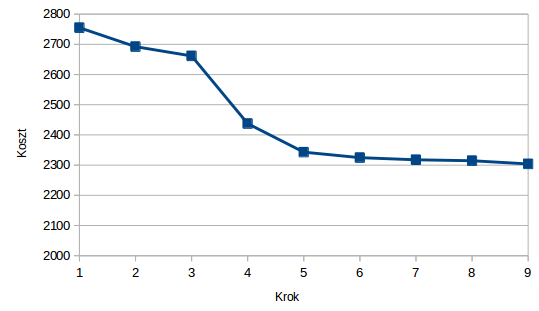
\includegraphics[width=\textwidth]{../image/dcg_regression.png}
  \caption{Spadek ceny w metodzie DCG}
  \label{fig:regression}
\end{figure}

Wyniki eksperymentu są zgodne z wynikami testu Gilmorea i Gomorego (\hyperref[sec:dcg]{rozdział~\ref*{sec:summary}})

\subsection{Wnioski}
Obie porównywane metody posiadają lepsze oraz gorsze cechy. Porównując metodę BF do DCG można określić że jest ona znacznie szybsza oraz daje bardziej homogeniczne rozkroje. Takie same długosci w jendym układzie powodują brak konieczności przestawiania noża podczas cięcia, skutkuje to mniejszym nakładem pracy podczas stosowania metody w warunkach rzeczywistych. Metoda ta odpowiednia jest do szybkiego prototypowania oraz szacowania kosztu. Przewagą metody DCG jest znaczna minimalizacja kosztu mimo większej liczby wykrojów i znacznie większego odpadu. Czas wykonania metody DCG powoduje iż, jest to metoda nieodpowiednia do planowania, lecz do określania konkretnych wykrojów. Jest to metoda bardziej oszczędna niż metoda BF.

Implementacja metody DCG użyta do testu, jest wariantem podstawowym zaprpopnowanym przez Gilmorea oraz Gomorego \cite{GilmoreGomoryV1Article}. Po wprowadzeniu usprawnień zaproponowanych w \cite{GilmoreGomoryV2Article} oraz optymalizacji implementacji, czas wykonania programu prawdopodobnie zostałby skrócony.
